%% ============================================================================
%% PhishGuard Defender -- IEEE conference paper (IEEEtran)
%% Compile on Overleaf with pdfLaTeX (Menu -> Compiler -> pdfLaTeX).
%% Bibliography: BibTeX with references.bib (Overleaf runs it automatically).
%% ============================================================================
\documentclass[conference]{IEEEtran}
\IEEEoverridecommandlockouts

\usepackage[T1]{fontenc}
\usepackage{cite}
\usepackage{amsmath,amssymb,amsfonts}
\usepackage{graphicx}
\usepackage{textcomp}
\usepackage{xcolor}
\usepackage{booktabs}
\usepackage{multirow}
\usepackage{array}
\usepackage{algorithm}
\usepackage{algpseudocode}
\usepackage{tikz}
\usetikzlibrary{arrows.meta,positioning,fit,calc,shapes.geometric}
\usepackage{url}
\usepackage[hidelinks]{hyperref}

\def\BibTeX{{\rm B\kern-.05em{\sc i\kern-.025em b}\kern-.08em
    T\kern-.1667em\lower.7ex\hbox{E}\kern-.125emX}}

\newcommand{\sys}{PhishGuard Defender}
\newcommand{\code}[1]{\texttt{\small #1}}

\begin{document}

\title{PhishGuard Defender: A Privacy-Preserving, Pre-Navigation Anti-Phishing
Protection System for Windows Endpoints and Chromium Browsers}

%% ---------------------------------------------------------------------------
%% TODO: replace the placeholders below with the real author names,
%% department, institution, city/country and e-mail addresses.
%% ---------------------------------------------------------------------------
\author{
\IEEEauthorblockN{Gollapalli Aakash Sudheendra}
\IEEEauthorblockA{\textit{Dept. of Computer Science} \\
\textit{and Engineering} \\
\textit{Amrita Vishwa Vidyapeetham}}
\and
\IEEEauthorblockN{Sanaka RajaSekhar}
\IEEEauthorblockA{\textit{Dept. of Computer Science} \\
\textit{and Engineering} \\
\textit{Amrita Vishwa Vidyapeetham}}
\and
\IEEEauthorblockN{Alla Rishi Venkatesh}
\IEEEauthorblockA{\textit{Dept. of Computer Science} \\
\textit{and Engineering} \\
\textit{Amrita Vishwa Vidyapeetham}}
}

\maketitle

%% ===========================================================================
\begin{abstract}
Phishing remains the most common initial-access vector in cyber attacks, and
users increasingly receive malicious links outside the e-mail client, through
web-based messengers such as WhatsApp Web, Telegram and Discord, collaboration
tools and documents. Blocklist-based browser protection reacts only after a URL
has been reported, while cloud reputation services send every visited URL to a
third party. This paper presents \sys{}, a real-time anti-phishing protection
system for Windows that combines a Manifest~V3 browser extension, an
authenticated localhost security service, and an Electron desktop protection
center around an explainable, offline phishing-scoring engine. The extension
intercepts top-level navigations through \code{webNavigation.onBeforeNavigate}
and captures cross-origin link clicks in the page's capture phase. It scores
each URL locally with an embedded port of the engine (19~structural features,
mean 0.145\,ms per URL) and redirects risky navigations to a local
interstitial. The remote page is never rendered. The local service adds
trusted-domain allow-listing, a configurable standard/strict policy,
fail-open or fail-closed behavior, time-boxed user bypasses, privacy redaction
of sensitive query parameters, and a server-sent-event channel that raises
native Windows notifications and an always-on-top alert window. On the
project's public-safe regression fixtures, the system blocks or warns on all
12~phishing URLs and allows 17 of 20~legitimate ones. Its three false
positives are documented branded-path cases. A cached decision is returned in
2.2\,ms and an uncached engine decision in a median of 11.7\,ms. All 214
automated unit, integration, and end-to-end tests pass. We describe the
architecture and its security model, and we discuss its limitations
candidly: URL-only features miss phishing pages whose URL looks clean, and
Manifest~V3 can only redirect a navigation, not hold it.
\end{abstract}

\begin{IEEEkeywords}
phishing detection, anti-phishing, browser extension, Manifest V3, endpoint
security, explainable security, privacy, Windows, Electron, URL analysis
\end{IEEEkeywords}

%% ===========================================================================
\section{Introduction}
\label{sec:intro}

Phishing continues to dominate the threat landscape. The Anti-Phishing Working
Group (APWG) observes on the order of a million unique phishing attacks per
quarter~\cite{apwg2024}, and the human element, including phishing and
pretexting, is involved in the majority of confirmed breaches~\cite{verizon2024}.
The delivery channel has also shifted. Malicious links are no longer confined
to e-mail and now arrive through web-based messaging (WhatsApp Web, Telegram,
Discord), shared documents, and collaboration platforms, where secure e-mail
gateways never inspect them.

Browsers already ship protection such as Google Safe Browsing~\cite{gsb} and
Microsoft Defender SmartScreen~\cite{smartscreen}. These services are
effective at scale, but they share two properties that motivate this work.
First, they are predominantly \emph{reactive}. A URL is blocked only after it
has been discovered, verified and propagated to a blocklist, and empirical
studies show that most phishing campaigns do their damage in the first hours,
before blocklists catch up~\cite{sheng2009,oest2019phishfarm,oest2020sunrise}.
Second, reputation look-ups that leave the device raise privacy and data
residency questions, especially in organizations whose URLs carry session
tokens or password-reset secrets.

The PhishGuard AI project~\cite{phishguardai} provides an explainable,
dependency-free and offline phishing-scoring engine for URLs and e-mail. Its
interfaces were developer-centric: a command-line tool, a Python API, a REST
endpoint, a GitHub Action and a browser demo. It could analyze a URL that a
user pasted in, but it could not \emph{stop} a user from opening one.

This paper presents \sys{}, the protection layer we built on top of that
engine so that it guards an ordinary Windows user in real time. Our
contributions are:

\begin{enumerate}
  \item \textbf{A four-tier pre-navigation protection architecture}
  (Section~\ref{sec:arch}). A Manifest~V3 extension, an authenticated
  localhost security service, the explainable Python engine, and an Electron
  desktop protection center cooperate so that a risky top-level navigation is
  replaced by a local interstitial before the remote page renders.
  \item \textbf{A defense-in-depth decision pipeline}
  (Section~\ref{sec:policy}). It combines an embedded offline scorer, a
  session cache, trusted-domain allow-listing, standard and strict policies,
  configurable fail-open and fail-closed behavior, and time-boxed,
  user-confirmed bypasses.
  \item \textbf{Privacy and local-service hardening}
  (Section~\ref{sec:security}): loopback-only binding, a 256-bit per-install
  authentication token, origin checks against drive-by requests from web
  pages, and redaction of sensitive query parameters before anything is
  logged.
  \item \textbf{Native Windows integration}
  (Section~\ref{sec:desktop}): a protection dashboard, security history,
  trusted-domain management, native notifications, an always-on-top alert
  window, a system-tray control and launch at sign-in.
  \item \textbf{An honest evaluation} (Section~\ref{sec:eval}) of detection
  decisions, latency and test coverage, together with the engine's published
  live-traffic and false-positive stress measurements, and a candid
  discussion of where the approach falls short (Section~\ref{sec:discussion}).
\end{enumerate}

%% ===========================================================================
\section{Background and Related Work}
\label{sec:related}

\subsection{Blocklists and Reputation Services}
Blocklists such as Google Safe Browsing~\cite{gsb}, SmartScreen~\cite{smartscreen}
and community feeds like OpenPhish~\cite{openphish} offer very high precision,
because every entry has been verified. Sheng~\emph{et~al.}~\cite{sheng2009}
showed, however, that most blocklists covered fewer than 20\% of phishing URLs
at hour zero. Oest~\emph{et~al.} measured how simple cloaking evades browser
blocklists~\cite{oest2019phishfarm} and how attack traffic peaks before
detection~\cite{oest2020sunrise}. Whittaker~\emph{et~al.}~\cite{whittaker2010}
described Google's large-scale classifier that feeds such lists. That
classifier runs in the provider's cloud, not on the endpoint.

\subsection{Heuristic and Learning-Based Detection}
URL-based classifiers avoid page retrieval and can therefore decide before a
page loads. Ma~\emph{et~al.}~\cite{ma2009beyond} showed that lexical and host
features of URLs identify malicious sites with high accuracy.
Sahingoz~\emph{et~al.}~\cite{sahingoz2019} and the URLNet deep
model~\cite{le2018urlnet} extended this line of work with natural-language
and character-level representations. Content-based systems such as
CANTINA~\cite{zhang2007cantina} reach higher recall on clean-looking URLs, but
they must fetch the page, which is precisely what pre-navigation protection
tries to avoid. Homograph and typosquatting attacks~\cite{gabrilovich2002}
motivate edit-distance~\cite{levenshtein1966} and internationalized-domain
features.

\subsection{Warnings and User Behavior}
A detector is only useful if its warning is heeded. Egelman~\emph{et~al.}
found that \emph{active}, interruptive phishing warnings are far more
effective than passive indicators~\cite{egelman2008}. Akhawe and Felt
measured click-through rates in the field and showed that warning design
strongly influences them~\cite{akhawe2013}. \sys{} follows these findings. It
uses a full-page interstitial, states the concrete reasons for the verdict,
and requires an explicit acknowledgement before the user can proceed.

\subsection{Positioning}
Table~\ref{tab:compare} positions \sys{} qualitatively. Its niche is
\emph{offline, explainable, pre-navigation} protection that keeps URLs on the
device and complements, rather than replaces, reputation services.

\begin{table}[t]
\centering
\caption{Qualitative comparison of protection approaches}
\label{tab:compare}
\setlength{\tabcolsep}{3pt}
\begin{tabular}{@{}lcccc@{}}
\toprule
Approach & Zero-hour & URL stays & Explains & Non-e-mail \\
         & coverage  & on device & verdict  & channels \\
\midrule
Cloud blocklist~\cite{gsb,smartscreen} & Low & Partial$^{a}$ & No & Yes \\
Secure e-mail gateway                 & Medium & No  & Partial & No \\
Content-based ML~\cite{zhang2007cantina} & High & No$^{b}$ & Rarely & Yes \\
PhishGuard AI CLI~\cite{phishguardai}  & Medium & Yes & Yes & Manual \\
\textbf{\sys{} (ours)}                 & \textbf{Medium} & \textbf{Yes} & \textbf{Yes} & \textbf{Yes} \\
\bottomrule
\multicolumn{5}{@{}l}{\footnotesize $^{a}$Hash-prefix protocols reduce but do not remove disclosure.}\\
\multicolumn{5}{@{}l}{\footnotesize $^{b}$Requires fetching the remote page.}
\end{tabular}
\end{table}

%% ===========================================================================
\section{Threat Model and Design Goals}
\label{sec:threat}

\textbf{Adversary.} A remote attacker who persuades the user to open a
credential-harvesting or malware-delivery URL. The link may arrive in an
e-mail, a web messenger, a document, or be typed or pasted into the address
bar. The attacker controls the URL and the page content, and may register new
domains, abuse free hosting platforms, use typosquatted or internationalized
names, raw IP addresses, or non-standard ports.

A second adversary is a \textbf{malicious web page} that tries to abuse the
local security service, for example by calling
\code{http://127.0.0.1:8766} from JavaScript to add itself to the trusted list
or to switch protection off.

\textbf{Out of scope.} Malware already running with the user's privileges.
Such code can tamper with any user-mode security product. We also exclude
compromised legitimate domains whose URLs are structurally indistinguishable
from benign ones. We discuss both in Section~\ref{sec:discussion}.

\textbf{Design goals.}
\begin{enumerate}
  \item[G1] \emph{Pre-navigation}: decide before the remote page is rendered.
  \item[G2] \emph{Privacy}: no URL leaves the device by default, and secrets in
        URLs are never persisted.
  \item[G3] \emph{Explainability}: every block states its reasons.
  \item[G4] \emph{Resilience}: protection degrades gracefully if a component
        is unavailable.
  \item[G5] \emph{Low latency}: safe browsing must not feel slower.
  \item[G6] \emph{User agency}: an informed user can proceed, and that choice
        is time-limited and recorded.
\end{enumerate}

%% ===========================================================================
\section{System Architecture}
\label{sec:arch}

Fig.~\ref{fig:arch} shows the four tiers and the path a click takes.

\begin{figure}[t]
\centering
\resizebox{\columnwidth}{!}{%
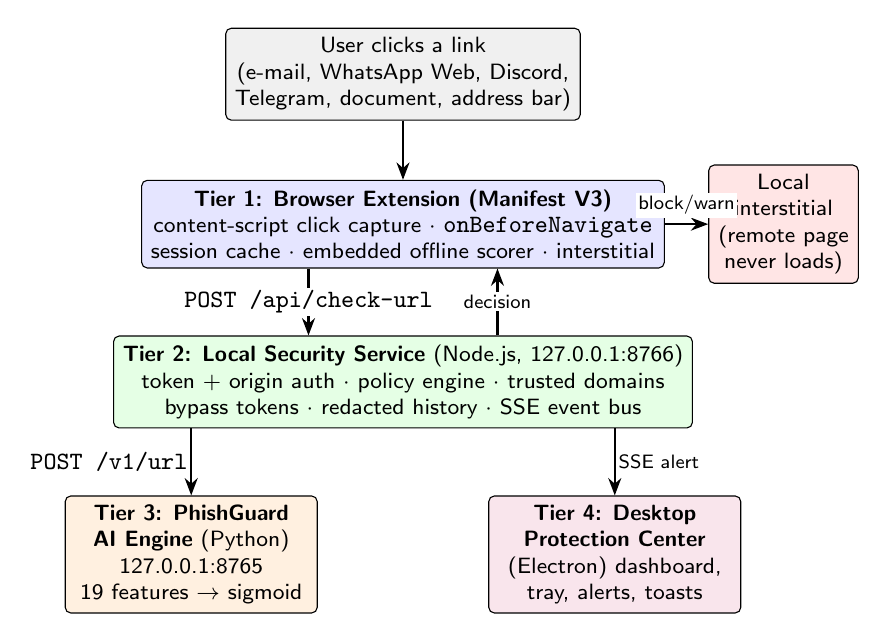
\begin{tikzpicture}[
  font=\sffamily\footnotesize,
  box/.style={draw, rounded corners=2pt, align=center, minimum width=3.2cm,
              minimum height=0.9cm, fill=#1},
  box/.default=white,
  arr/.style={-{Stealth[length=2.2mm]}, thick},
  lbl/.style={font=\sffamily\scriptsize, align=center, fill=white, inner sep=1pt}
]
  \node[box=gray!12] (user) {User clicks a link\\(e-mail, WhatsApp Web, Discord,\\Telegram, document, address bar)};
  \node[box=blue!10, below=0.75cm of user, minimum width=6.4cm] (ext)
    {\textbf{Tier 1: Browser Extension (Manifest V3)}\\
     content-script click capture $\cdot$ \code{onBeforeNavigate}\\
     session cache $\cdot$ embedded offline scorer $\cdot$ interstitial};
  \node[box=green!10, below=0.85cm of ext, minimum width=6.4cm] (svc)
    {\textbf{Tier 2: Local Security Service} (Node.js, 127.0.0.1:8766)\\
     token + origin auth $\cdot$ policy engine $\cdot$ trusted domains\\
     bypass tokens $\cdot$ redacted history $\cdot$ SSE event bus};
  \node[box=orange!12, below left=0.85cm and -2.6cm of svc] (eng)
    {\textbf{Tier 3: PhishGuard}\\\textbf{AI Engine} (Python)\\127.0.0.1:8765\\19 features $\to$ sigmoid};
  \node[box=purple!10, below right=0.85cm and -2.6cm of svc] (desk)
    {\textbf{Tier 4: Desktop}\\\textbf{Protection Center}\\(Electron) dashboard,\\tray, alerts, toasts};
  \node[box=red!10, right=0.55cm of ext.east, minimum width=1.9cm, anchor=west] (inter)
    {Local\\interstitial\\(remote page\\never loads)};

  \draw[arr] (user) -- (ext);
  \draw[arr] ([xshift=-12mm]ext.south) -- node[lbl]{\code{POST /api/check-url}} ([xshift=-12mm]svc.north);
  \draw[arr] ([xshift=12mm]svc.north) -- node[lbl]{decision} ([xshift=12mm]ext.south);
  \draw[arr] (svc.south -| eng.north) -- node[lbl,left]{\code{POST /v1/url}} (eng.north);
  \draw[arr] (svc.south -| desk.north) -- node[lbl,right]{SSE alert} (desk.north);
  \draw[arr] (ext.east) -- node[lbl,above=2pt]{block/warn} (inter.west);
\end{tikzpicture}}
\caption{Architecture of \sys{}. A risky top-level navigation is replaced by an
extension-local interstitial; every component communicates only over the
loopback interface.}
\label{fig:arch}
\end{figure}

\subsection{Tier 1: Manifest V3 Browser Extension}
\label{sec:ext}
Chromium's Manifest~V3~\cite{mv3} removed blocking \code{webRequest}
listeners for most extensions, so an extension can no longer hold a request
open while it waits for an asynchronous verdict. \sys{} therefore uses two
complementary interception points.

\emph{(i) Navigation interception.} A listener on
\code{chrome.webNavigation.onBeforeNavigate}~\cite{webnav} fires for every
top-level (\code{frameId}\,$=$\,0) HTTP(S) navigation, including typed URLs,
bookmarks and links opened from other applications. The service worker first
consults a five-minute session cache. It then runs the \emph{embedded offline
scorer}, a JavaScript port of the engine that is bundled with the extension
together with the Mozilla Public Suffix List~\cite{psl}. If that scorer flags
the URL, the tab is immediately updated to the packaged page
\code{pages/interstitial.html}, which receives the target URL and decision.
The local service is still notified in the background so that the desktop
alert fires. If the offline scorer does not flag the URL, the service is
queried asynchronously and the tab is redirected if the authoritative verdict
is \code{block} or \code{warn}.

\emph{(ii) Click capture in messaging pages.} A content script injected at
\code{document\_start} registers a \emph{capture-phase} click listener. For
any cross-origin link it synchronously calls \code{preventDefault()} and
\code{stopImmediatePropagation()}, asks the service worker for a decision and
then either opens the link with \code{noopener,noreferrer} or shows an in-page
modal. Because the default action is cancelled synchronously, this path
genuinely holds the navigation until a verdict exists. It covers single-page
applications such as WhatsApp Web, Telegram Web, Discord, Gmail and Outlook
on the web, where links are often opened by script.

The interstitial and the in-page modal show the risk score, the
classification and human-readable reasons derived from the triggered
features. Following~\cite{egelman2008,akhawe2013}, the default action is
\emph{Close (do not open website)}. Proceeding requires ticking an ``I
understand the risk'' box first.

\subsection{Tier 2: Local Security Service}
A dependency-free Node.js HTTP service bound to \code{127.0.0.1:8766}
mediates every decision. It exposes \code{/api/check-url}, \code{/api/stats},
\code{/api/history}, \code{/api/settings}, \code{/api/trusted},
\code{/api/bypass}, \code{/api/cancel-navigation} and an \code{/api/events}
server-sent-event (SSE) stream. The service manages the Python engine's
life cycle. It probes \code{/healthz}, spawns \code{phishguard.py serve} on
demand, and falls back to a one-shot CLI invocation when the HTTP engine is
unreachable. Settings, trusted domains and history are kept in atomically
written JSON files.

\subsection{Tier 3: Explainable Detection Engine}
\label{sec:engine}
The engine~\cite{phishguardai} extracts structural features from the URL
string alone, with no DNS lookup or page fetch. The features include
host-and-path length (capped at 80 characters, with the query string
excluded), query-parameter count, public-suffix-aware subdomain depth, IP
literal hosts, explicit ports, HTTPS, nine high-risk TLDs, matches against 30
credential and brand keywords, digit and special-character ratios,
character entropy, punycode and Unicode host labels, Levenshtein distance to
popular brands~\cite{levenshtein1966}, and free hosting platforms. Optional,
opt-in signals cover redirect chains (compared at the eTLD+1 level) and
domain age obtained via RDAP~\cite{rfc9083}. With weights $w_i$ and feature
values $x_i$, the score is
\begin{equation}
  p = \sigma\!\Big(k\big(b + \textstyle\sum_i w_i x_i\big)\Big),
  \qquad \sigma(z)=\frac{1}{1+e^{-z}},
  \label{eq:score}
\end{equation}
with bias $b=-1.30$ and steepness $k=2.5$. The verdict is
\begin{equation}
  v(p)=
  \begin{cases}
    \textsc{Phishing}   & p \ge 0.75,\\
    \textsc{Suspicious} & 0.55 \le p < 0.75,\\
    \textsc{Safe}       & p < 0.55.
  \end{cases}
  \label{eq:verdict}
\end{equation}
The weights are hand-tuned and documented, not learned. Table~\ref{tab:weights}
lists the most influential ones. Every non-zero term $w_i x_i$ can be shown
to the user, which gives the explainability required by goal~G3. A
cross-language parity test keeps the embedded JavaScript scorer identical to
the Python reference implementation.

\begin{table}[t]
\centering
\caption{Most influential URL feature weights in the engine}
\label{tab:weights}
\begin{tabular}{@{}lrl@{}}
\toprule
Feature & $w_i$ & Rationale \\
\midrule
\code{has\_ip\_address}          & $+0.90$ & IP literal instead of a name \\
\code{has\_opaque\_hostname\_label}& $+0.90$ & generated-looking host label \\
\code{suspicious\_tld}           & $+0.70$ & \code{.xyz}, \code{.tk}, \code{.top}, \dots \\
\code{on\_free\_hosting\_platform} & $+0.70$ & disposable subdomain hosting \\
\code{typosquatting\_score}      & $+0.65$ & small edit distance to a brand \\
\code{digit\_ratio}              & $+0.60$ & digit-heavy host/path \\
\code{has\_port}                 & $+0.40$ & non-standard port \\
\code{phishing\_keywords}        & $+0.25$ & per matched keyword \\
\code{subdomain\_count}          & $+0.18$ & per label above eTLD+1 \\
\code{has\_https}                & $-0.20$ & TLS present \\
\bottomrule
\end{tabular}
\end{table}

\subsection{Tier 4: Windows Desktop Protection Center}
\label{sec:desktop}
An Electron~\cite{electron} application embeds the local service in its main
process and subscribes to policy alerts. Its renderer windows run with
\code{contextIsolation} enabled, \code{nodeIntegration} disabled, and a
narrow \code{preload} bridge, as recommended by Electron's security
guidance~\cite{electronsec}. The center provides:
(a)~a dashboard with scanned, blocked, suspicious and safe counters and the
connection status of the extension and the engine;
(b)~a searchable and filterable security history;
(c)~trusted-domain management;
(d)~settings for real-time protection, notifications, the alert pop-up,
policy mode, fail mode and auto-start;
(e)~a native Windows toast and an always-on-top alert window for every
blocked or warned navigation, whose \emph{Close} button propagates a
\code{CANCEL\_NAVIGATION} event back to the extension over SSE so that the
offending tab is closed; and
(f)~a system-tray icon with a protection toggle and launch at sign-in.
\code{electron-builder} packages the application as an NSIS installer.

%% ===========================================================================
\section{Decision Pipeline and Policy}
\label{sec:policy}

Algorithm~\ref{alg:policy} gives the service-side evaluation order. The
order is deliberate. User intent (protection off, trusted domain, explicit
bypass) is honored before any scoring, and cached results short-circuit the
engine to meet goal~G5.

\begin{algorithm}[t]
\caption{Service-side URL evaluation}
\label{alg:policy}
\begin{algorithmic}[1]
\Require URL $u$, settings $S$
\If{$u$ is not \texttt{http(s)} \textbf{or} $\neg S.\mathit{realTime}$}
  \State \Return \textsc{allow}
\EndIf
\State $d \gets \mathrm{eTLD{+}1}(u)$
\If{$d \in \mathit{Trusted}$} \Return \textsc{allow} \EndIf
\If{active bypass for $u$ or $d$} \Return \textsc{allow} (bypassed) \EndIf
\If{$\mathit{cache}[u]$ is fresh} \Return $\mathit{cache}[u]$ \EndIf
\State $(v,p,\mathbf{x}) \gets \textsc{Engine}(u)$ \Comment{on error: fail mode}
\If{$v=\textsc{Phishing}$} $a \gets \textsc{block}$
\ElsIf{$v=\textsc{Suspicious}$}
  \State $a \gets \textsc{block}$ \textbf{if} $S.\mathit{mode}=\textit{strict}$ \textbf{else} \textsc{warn}
\Else\ $a \gets \textsc{allow}$
\EndIf
\State cache $(u,a)$ for $S.\mathit{ttl}$; log $\textsc{Redact}(u)$
\If{$a\neq\textsc{allow}$} broadcast SSE alert \EndIf
\State \Return $(a, v, \mathrm{round}(100p), \mathrm{reasons}(\mathbf{x}))$
\end{algorithmic}
\end{algorithm}

\textbf{Policy modes.} In \emph{standard} mode, \textsc{Suspicious} URLs
produce a warning and \textsc{Phishing} URLs are blocked. \emph{Strict} mode
blocks both, which suits high-risk users or managed devices.

\textbf{Failure handling (G4).} If the engine is unreachable,
\emph{fail-open} (the default) allows the navigation, marks the verdict
\textsc{Unknown} and relies on the extension's embedded scorer, which is
still active. \emph{Fail-closed} blocks unverified URLs with a
\textsc{Suspicious} verdict. If the whole service is down, the extension
falls back to its offline scorer, so obviously malicious URLs are still
blocked without any running service.

\textbf{Bypass (G6).} \emph{Proceed anyway} grants a bypass for the URL and
its registrable domain that expires after 600\,s by default. The bypass is
logged, which avoids permanent ``click-once, trust-forever'' exceptions.

%% ===========================================================================
\section{Security and Privacy Design}
\label{sec:security}

A localhost service is an attractive target: any web page can attempt
\code{fetch()} requests to \code{127.0.0.1}. Table~\ref{tab:threats} maps
threats to mitigations.

\begin{table}[t]
\centering
\caption{Threats against the local service and mitigations}
\label{tab:threats}
\setlength{\tabcolsep}{3pt}
\begin{tabular}{@{}p{0.42\columnwidth}p{0.53\columnwidth}@{}}
\toprule
Threat & Mitigation \\
\midrule
Remote host reaches the service & Bound to \code{127.0.0.1} only \\
Web page calls the API (CSRF-style) & 256-bit token in \code{X-PhishGuard-Auth}; non-extension, non-loopback \code{Origin} rejected (403); CORS echoes only allowed origins \\
Web page reads the token & \code{/api/token} answers loopback sockets only; a cross-origin page cannot read the response under CORS \\
Secrets leak into history & Sensitive query parameters and long values replaced by \code{[REDACTED]} before storage \\
Oversized request (DoS) & 1\,MiB request-body limit \\
Renderer compromise in desktop app & \code{contextIsolation}, no \code{nodeIntegration}, minimal preload API \\
\bottomrule
\end{tabular}
\end{table}

\textbf{Token authentication.} At first start the service generates a
token with \code{crypto.randomBytes(32)}, stores it with file mode
\code{0600}, and requires it, as a header or as a bearer token, on every
endpoint except \code{/healthz}.

\textbf{Origin enforcement.} Requests whose \code{Origin} header is neither
\code{chrome-extension://}, \code{moz-extension://} nor a loopback origin are
rejected, and the CORS headers echo only those origins. A malicious page
therefore cannot change settings or add trusted domains even if it guesses
the endpoint.

\textbf{Privacy by redaction (G2).} Before an event is written, parameters
named \code{token}, \code{access\_token}, \code{auth}, \code{password},
\code{key}, \code{code}, \code{session\_id}, \code{jwt}, \code{secret} and
similar names, and any value longer than 40 characters, are replaced. For
example, \url{https://login.example.com/verify?token=s3cr3t&user=john}
becomes \url{https://login.example.com/verify?token=[REDACTED]&user=john}. By default no URL is sent to
any external service. The engine's RDAP domain-age check is the only network
feature, and it is opt-in.

%% ===========================================================================
\section{Implementation}
\label{sec:impl}

Table~\ref{tab:impl} summarizes the code base. The extension, service and
desktop application are new in this work. The engine is reused from
PhishGuard AI v0.5.1~\cite{phishguardai}. Apart from Electron, all components
use only the standard libraries of Python~3.10+ and Node.js~18+. The engine
runs as a separate local process, so a crash in the scorer cannot take the
service down.

\begin{table}[t]
\centering
\caption{Implementation summary}
\label{tab:impl}
\setlength{\tabcolsep}{4pt}
\begin{tabular}{@{}llr@{}}
\toprule
Component & Technology & LoC$^{\dagger}$ \\
\midrule
Browser extension (MV3)   & JavaScript, HTML/CSS     & 1\,266 \\
Local security service    & Node.js (stdlib only)    & 1\,226 \\
Desktop protection center & Electron 28              & 422 \\
Detection engine (reused) & Python 3 (stdlib only)   & 2\,042 \\
Integration/E2E tests     & Node.js \code{assert}, \code{unittest} & -- \\
\bottomrule
\multicolumn{3}{@{}l}{\footnotesize $^{\dagger}$Main logic files, excluding renderer markup and styles.}
\end{tabular}
\end{table}

%% ===========================================================================
\section{Evaluation}
\label{sec:eval}

We evaluate four questions. \textbf{RQ1:} Does the end-to-end system reach
the correct block, warn or allow decision? \textbf{RQ2:} Is the added latency
acceptable? \textbf{RQ3:} How does the underlying engine behave on live
traffic? \textbf{RQ4:} Do the protection mechanisms work as specified?

\textbf{Setup.} Measurements were taken on a consumer Windows~11 laptop
(Python~3.12.4, Node.js~24.21) with the service in standard mode, fail-open,
and the default trusted list. To avoid contacting live phishing
infrastructure, RQ1 and RQ2 use the project's three public-safe fixtures (32
URLs in total). Phishing samples are either synthetic or drawn from the
CC-BY URL-Phish dataset~\cite{urlphish} and neutralized to the reserved
\code{.example} TLD.

\subsection{RQ1: Decision Correctness}
Table~\ref{tab:decisions} reports the decisions. The embedded offline scorer
classifies the regression and public fixtures perfectly (12~TP, 12~TN). The
service blocks 6 and warns on 6 of the 12 phishing URLs, so \emph{every}
phishing URL is intercepted before rendering. In strict mode, all 12 would be
blocked. Of the 20 legitimate URLs, 17 are allowed. The three false positives
come from the \emph{branded-path} stress fixture, which deliberately contains
realistic legitimate shapes that resemble phishing:
\code{accounts.<brand>/signin} and \code{secure.<brand>/login} (warned), and
\code{/support/account/security/verify-identity} (blocked). These are known,
documented limitations of URL-only scoring, not regressions.

\begin{table}[t]
\centering
\caption{End-to-end decisions on public-safe fixtures (standard mode)}
\label{tab:decisions}
\setlength{\tabcolsep}{3.5pt}
\begin{tabular}{@{}lccccc@{}}
\toprule
Fixture & $n$ & Offline TP/TN/FP/FN & Block & Warn & Allow \\
\midrule
Regression        & 14 & 7 / 7 / 0 / 0 & 6 & 1 & 7 \\
Public (URL-Phish)& 10 & 5 / 5 / 0 / 0 & 0 & 5 & 5 \\
Branded-path      &  8 & 0 / 5 / 3 / 0 & 1 & 2 & 5 \\
\midrule
\textbf{Total}    & \textbf{32} & \textbf{12 / 17 / 3 / 0} & \textbf{7} & \textbf{8} & \textbf{17} \\
\bottomrule
\end{tabular}
\end{table}

\subsection{RQ2: Latency}
Table~\ref{tab:latency} shows the latencies. The embedded scorer needs
0.145\,ms per URL on average, measured over 64\,000 evaluations. This
pre-check is what makes interception of obviously malicious URLs immediate.
An uncached service decision, which includes the HTTP hop to the Python
engine, has a median of 11.7\,ms. Its tail (p95 277\,ms) comes from
occasional engine-side overheads. A cached decision takes 2.2\,ms. Both
service paths are well below the hundreds of milliseconds a typical page
needs to load.

\begin{table}[t]
\centering
\caption{Decision latency (ms)}
\label{tab:latency}
\begin{tabular}{@{}lrrrr@{}}
\toprule
Path & $n$ & Mean & p50 & p95 \\
\midrule
Embedded offline scorer (in-process) & 64\,000 & 0.145 & -- & -- \\
Service, uncached (engine call)       & 32 & 36.26 & 11.66 & 276.76 \\
Service, cached                       & 32 & 2.21 & 2.17 & 2.86 \\
\bottomrule
\end{tabular}
\end{table}

\subsection{RQ3: Engine on Live Traffic}
The engine's maintainers report string-only evaluations against
currently live phishing URLs from OpenPhish~\cite{openphish} and legitimate
domains from the Tranco ranking~\cite{tranco}. We summarize the independently
reconfirmed run~\cite{phishguardai} in Table~\ref{tab:live}. No false positive
occurred on 1\,000 top Tranco root URLs. Recall on 300 live phishing URLs is
moderate: 55.7\% flagged and 34.0\% strict \textsc{Phishing}. It rises with
opt-in domain age. On 30\,000 realistic login, reset and verification URL
shapes built from 3\,000 legitimate domains, the flagged rate is 21.4\% (10.3\%
strict). This shows that the warn tier in standard mode is important for
keeping false blocks low.

\begin{table}[t]
\centering
\caption{Engine evaluation on live and stress data (from~\cite{phishguardai})}
\label{tab:live}
\setlength{\tabcolsep}{3pt}
\begin{tabular}{@{}lcc@{}}
\toprule
Metric & Offline & + Domain age \\
\midrule
Recall, flagged (300 OpenPhish URLs)    & 55.7\% & 59.0\% \\
Recall, strict \textsc{Phishing}       & 34.0\% & 34.7\% \\
FP, Tranco top-1\,000 root URLs        & 0 / 1\,000 & 0 / 300 \\
FP stress, flagged (30\,000 URL shapes)& 21.4\% & 16.9\%$^{*}$ \\
FP stress, strict \textsc{Phishing}    & 10.3\% & 6.5\%$^{*}$ \\
\bottomrule
\multicolumn{3}{@{}l}{\footnotesize $^{*}$150-domain subsample (1\,500 URLs).}
\end{tabular}
\end{table}

\subsection{RQ4: Functional Verification}
All automated suites pass on the measurement machine (Table~\ref{tab:tests}).
The nine service integration tests cover health discovery, rejection of
missing and invalid tokens (HTTP~401), statistics, trusted-domain
short-circuiting, phishing blocking with a risk score of at least 75 and
non-empty reasons, query-parameter redaction, redacted history persistence,
and the bypass workflow. The six end-to-end tests drive the real Python
engine through the service and assert block, warn and allow outcomes,
allow-listing, redaction and bypass. The manual acceptance scenario in Chrome
and Edge uses two URLs. \code{https://www.google.com} scores
$p=0.168$ (\textsc{Safe}) and loads normally.
\code{http://paypa1-secure-login.xyz/verify} scores $p=0.951$
(\textsc{Phishing}). Its tab is replaced by the interstitial with a 95\% risk
score, the reasons ``suspicious TLD'', ``3 credential keywords'', ``high
entropy'' and ``no HTTPS'', and a native Windows alert.

\begin{table}[t]
\centering
\caption{Automated test results}
\label{tab:tests}
\begin{tabular}{@{}lrl@{}}
\toprule
Suite & Tests & Result \\
\midrule
Engine unit tests (Python)          & 199 & pass$^{\ddagger}$ \\
Local service integration (Node.js) & 9   & pass \\
End-to-end protection (Python)      & 6   & pass \\
\midrule
\textbf{Total}                      & \textbf{214} & \textbf{all pass} \\
\bottomrule
\multicolumn{3}{@{}l}{\footnotesize $^{\ddagger}$Includes one tracked expected failure and JS/Python parity tests.}
\end{tabular}
\end{table}

%% ===========================================================================
\section{Discussion and Limitations}
\label{sec:discussion}

\textbf{URL-only signal.} The largest limitation is inherited from the
engine. About three quarters of missed live phishing URLs are bare root
URLs on fresh or compromised domains, which carry no lexical signal at all.
Closing this gap needs signals that remain privacy-compatible, such as
on-device page-content analysis after the page has loaded, visual brand
similarity, or local caching of a downloaded blocklist. \sys{} is designed to
\emph{complement} Safe Browsing and SmartScreen, not to replace them.

\textbf{Manifest~V3 timing.} Without blocking \code{webRequest}, the
\code{onBeforeNavigate} path \emph{redirects} the tab instead of holding the
request. For URLs that the embedded scorer flags, the redirect is issued at
once. For URLs that only the service flags, a short race exists in which the
browser may begin loading. In practice both tiers use the same model, so they
rarely disagree, and the content-script path holds clicks synchronously. A
declarative-rule fallback built on \code{declarativeNetRequest} dynamic rules
for known-bad domains would close this window.

\textbf{Local trust boundary.} Any local process can obtain the token from
\code{/api/token}. That is consistent with our threat model, which excludes
local malware, but OS-level secret storage such as Windows DPAPI, or native
messaging, would be stronger. The SSE stream also accepts the token as a query
parameter, a convenience that should be removed in favor of headers only.

\textbf{Usability.} Warning fatigue is real~\cite{akhawe2013}. The
standard-mode warn tier, the trusted list and time-boxed bypasses aim to keep
false blocks rare, but a user study measuring click-through and perceived
burden is future work.

\textbf{Evaluation scope.} The end-to-end fixtures are small and
public-safe by design. They detect regressions but do not measure accuracy at
population level.

%% ===========================================================================
\section{Conclusion and Future Work}
\label{sec:conclusion}

We presented \sys{}, a Windows anti-phishing system that turns an
explainable, offline URL-scoring engine into real-time, pre-navigation
protection across the browser, web messengers and the desktop. Four tiers,
an authenticated loopback service and a defense-in-depth policy keep URLs on
the device, explain every block, and degrade gracefully. The system
intercepts every phishing URL in our public-safe fixtures and adds only a few
milliseconds of latency. Future work includes on-device content and visual
similarity models, \code{declarativeNetRequest} fallback rules, DPAPI-backed
secrets, a Firefox port, enterprise policy deployment through Group Policy or
Intune, and a controlled user study.

%% ===========================================================================
\section*{Acknowledgment}
The detection engine is the open-source PhishGuard AI project by
O.~Adeyan~\cite{phishguardai}, released under the MIT license. We thank its
maintainers and the creators of the URL-Phish dataset~\cite{urlphish}.

\bibliographystyle{IEEEtran}
\bibliography{references}

\end{document}
